\documentclass[utf8, a4paper, 12pt]{article}
\usepackage[right=2.50cm,left=2.50cm,top=2cm, bottom=2cm]{geometry}
\usepackage{indentfirst} 
\setlength{\parindent}{2em}
\title{Graph Drawing Contest 2020}
\author{Kunhao ZHENG\qquad Yuyang ZHAO }
\date{January 2020}
\usepackage{algorithm}
\usepackage{algorithmic}
\usepackage{subfigure}
\usepackage{graphicx}
\usepackage{booktabs}
\usepackage{threeparttable}
 \usepackage{multirow} 
\renewcommand{\arraystretch}{1.5}
\renewcommand{\algorithmicrequire}{ \textbf{Input:}}
\renewcommand{\algorithmicensure}{ \textbf{Output:}} 
\begin{document}

   
\maketitle

\section{Problem Description}
\indent A  \textit{straight-line upward grid drawing} is a 2D drawing in which the following conditions are satisfied:\\
(1) For each edge, the target vertex should have a strictly higher y-coordinate than the source vertex.\\
(2) For each edge, neither the target vertex nor the source vertex could be on the line segment of another edge.\\
(3) The graph is embedded on the input grid: the x-coordinate and y-coordinate of the vertices must be integers on a grid of size [0..width]$\times$[0..height].\\
~\\
\indent Given the input graph in JSON format, which contains a list of vertices and a list of oriented edges, we try to firstly check the validity of a drawing and compute the number of drawing; and then construct a valid drawing by moving the nodes in the grid; finally minimize the number of crossing based on a valid drawing.\\

\section{Algorithm}
\subsection{Checking the validity of a drawing}
Among the three conditions, the most difficult one to verify is to check whether the target vertex or the source vertex are on the line segment of another edge, so we introduce the lemme below:\\
\textit{Lemme: P(x,y) is on the segment of endpoints $(x_{1},y_{1}),(x_{2},y_{2})$ (endpoints included), if and only if
\begin{itemize}
    \item $(x-x_{1})\times(y-y_{2})=(x-x_{2})\times(y-y_{1})$
    \item $(x-x_{1})\times(x-x_{2})\leq 0$
    \item $(y-y_{1})\times(y-y_{2})\leq 0$
\end{itemize}}

\begin{algorithm}
\caption{Check the validity of a drawing} 
\begin{algorithmic}
\FOR{each $e\in G$}
\STATE verify $y_{source}\textless y_{target}$;\
\STATE verify neither source vertex nor target vertex is on the line segment of another edge;\
\STATE verify the vertices are in the grid;\
\IF{at least one condition is not satisfied}
\RETURN false
\ENDIF
\ENDFOR
\RETURN true
\end{algorithmic}
\end{algorithm}
~\\
\indent And then we are supposed to calculate the number of crossing. We introduce the lemme below to judge whether the two edges have a crossing.\\
\textit{Lemme: the edge $P_{1}P_{2}$ and the edge $Q_{1}Q_{2}$ have a crossing, if and only if
\begin{itemize}
    \item $(\vec{P_{1}P_{2}}\times\vec{P_{1}Q_{1}})\cdot(\vec{P_{1}P_{2}}\times\vec{P_{1}Q_{2}})\leq0$ 
    \item $(\vec{Q_{1}Q_{2}}\times\vec{Q_{1}P_{1}})\cdot(\vec{Q_{1}Q_{2}}\times\vec{Q_{1}P_{2}})\leq0$ 
\end{itemize}}

\begin{algorithm}
\caption{Compute the number of crossing} 
\begin{algorithmic}
\STATE $counter \Leftarrow 0$ 
\FOR{each $e_{1}\in G$}
\FOR{each $e_{2}\in G$}
\IF{$e_{1}=e_{2}$}
\STATE continue
\ELSE
\IF {$e_{1}$ and $e_{2}$ have a crossing}
\STATE  $counter \Leftarrow counter+1 $
\ENDIF
\ENDIF
\ENDFOR
\ENDFOR
\RETURN counter
\end{algorithmic}
\end{algorithm}
\subsection{Compute a valid drawing}
\indent To compute a valid drawing, firstly we compute a \textit{topological ordering} of the graph with a DFS traversal, and then we decide the position of each node according to this ordering. Recall the definition of \textit{topological ordering} as follows.\\
\textit{Definition (topological ordering):\\
Topological Sorting for Directed Acyclic Graph (DAG) is a linear ordering of vertices such that for every directed edge, the source vertex comes before the target vertex in the ordering.}
\begin{algorithm}
\begin{algorithmic}[1]
\caption{Topological Order}
\REQUIRE ~~\\ 
Directed Acyclic Graph G=(V,E);\\
\ENSURE ~~\\ 
List of vertices in topological ordering;
\STATE  Create a temporary stack and a boolean array named as visited[ ].
\STATE  Mark all the vertices as not visited i.e. initialize visited[ ] with 'false' value.
\STATE  Call the recursive helper function topologicalSortUtil() to store Topological Sort starting from all vertices one by one.
\STATE Define the function topologicalSortUtil():
\begin{itemize}
\item Mark the current node as visited.
\item Recall for all the successors of this vertex.
\item Push current vertex to stack which stores result.
\end{itemize}
\STATE Print contents of stack.
 \end{algorithmic}
\end{algorithm}\\
~\\
\indent After sorting the vertices in \textit{topological order}, we are going to decide the position of each node according to this order. In this way, for each node, we place all of its predecessors before deciding its position so that the condition about the relationship of y-coordinates can be satisfied easily. \\
\indent The principal idea is that for each node, we compute the maximum y-coordinate of its predecessors, note $y_{max}$ and we start to try to place the node on the position [0,$y_{max}+1$], and to check the validity of the present drawing. If not, we place the node on [1,$y_{max}+1$] and repeat the process until find a valid position. (If all of points with $y_{max}+1$ can't satisfy the conditions, we start to try $y_{max}+2$ ). \\

\begin{algorithm}
\caption{Compute a valid drawing} 
\begin{algorithmic}
\REQUIRE ~~\\ 
A given drawing G in JSON format;\\
List of vertices in topological ordering L;\\
\ENSURE ~~\\ 
A valid drawing $G^\prime$;\\
\IF{ G is a valid drawing}
\RETURN G
\ENDIF
\STATE Creat a blank drawing $G^\prime$
\FOR{Vertices $v \in G$}
\STATE $y_{max}\Leftarrow$ maximum y-coordinate among predecessors of $v$
\STATE $x\Leftarrow 0$
\STATE $y\Leftarrow y_{max}+1$
\WHILE{the present drawing isn't valid}
\IF{$x<Width-1$}
\STATE$x\Leftarrow x+1$
\ELSE
\STATE $x\Leftarrow 0$
\STATE $y\Leftarrow y+1$
\ENDIF
\STATE place $v$ on the position $[x,y]$
\ENDWHILE
\ENDFOR

\RETURN $G^{\prime}$
\end{algorithmic}
\label{initial}
\end{algorithm}

\subsection{Minimize the number of crossing}
In order to minimize the number of crossing, we have two different method: force-directed layouts and local search heuristic.\\
~\\
\textbf{Method 1: Force-directed layouts}\\
\indent In this model, vertices can be seen as particles of a physical system that evolves under the action of forces exerced on the vertices. We define three kinds of forces as follows:
\begin{itemize}
\item For any pair of vertices $(u,v)$, there exists a repulsive force.
$$F=\frac{-CK^{2}(\mathbf{x}(v)-\mathbf{x}(u))}{{ \left[ \left\| \mathbf{x}(v)-\mathbf{x}(u) \right\|\right]  }^{2}}$$

\item Between the adjacent vertices $(u,v)$, there exists an attractive force.
$$F=\frac{\left[ \left\| \mathbf{x}(v)-\mathbf{x}(u) \right\| \right] }{K}(\mathbf{x}(v)-\mathbf{x}(u))$$   

\item For any pair of edges of the same source vertex $(\vec{AB},\vec{AC})$,with an intersection angle $\theta$,  there exists a repulsive force in the horizontal direction.
$$F=(\alpha({\tan}^{-1}(\frac{\left[ \left\|\vec{AB}\right\| \right]}{\beta})+{\tan}^{-1}(\frac{\left[  \left\|\vec{AC}\right\| \right] }{\beta}))+\gamma \cot(\frac{\theta}{2}))$$

\end{itemize}
~\\
\indent In order to remain a valid drawing, after determining the new position of the present vertex. If the new position is higher (have a bigger y-coordinate) than the old one, we augment all of vertices higher than it in the old drawing by the same length.  If the new position is lower (have a smaller y-coordinate) than the old one, we diminish all of vertices lower than it in the old drawing by the same length. Then we check the validity of the present drawing, if it is valid, we remain this change.  \\
~\\
\textbf{Method 2: Local search heuristic}\\
\indent Local search is a heuristic method for solving computationally hard optimization problems. Local search algorithms move from solution to solution in the space of candidate solutions (the search space) by applying local changes, until a solution deemed optimal is found or a time bound is elapsed.\\
\indent In this problem, each time in the iteration we find the edge who has the biggest crossing numbers by using a priority queue. Then we do a local research by moving the source vertex and the target vertex of this edge, to determine the best position (diminish largely the number of crossing). In each iteration we will reduce both the search range and the search step by half. Thus we need two constant described the initial search range and the initial step length in the pseudo-code $C_{step}$ and $C_{range}$. For some large inputs, we set $C_{step} = 10$ and $C_{range}=5$. On the contrary, if the size of the graph is small, we set $C_{step}=height$ and $C_{range}=1$ by doing a global research to find the best new position. Finally we do the iteration for the new drawing.

\begin{algorithm}
\caption{Local research heuristic}
\begin{algorithmic}
\REQUIRE~~\\
\STATE Height, Weight: criterion of type of research;\\
\STATE A 2D valid drawing G of size $G_{height}\times G_{width}$;\\
\ENSURE~~\\
\STATE A valid drawing $G^\prime$;\\
\STATE Find the edge which most contributes to the number of crossing\\
\STATE $counter\Leftarrow$ the number of crossing of $G$\\
\IF{$G_{height}<$Height \AND $G_{width}<Width$}
\STATE $step\Leftarrow Height/C_{step}$,\\
\STATE $Xrange=Width, Yrange=Height,$\\
\STATE$ (Xnew,Ynew)=(Width/C_{range},Height/C_{range})$\\
\WHILE{$step>0$}
\STATE Find and update the best position among $(\{Xnew+\mathrm{N}step\}\cap[Xnew-Xrange/2,Xnew+Xrange/2],\{Ynew+\mathrm{N}step\}\cap[Ynew-Yrange/2,Ynew+Yrange/2])$\\
\STATE $step\Leftarrow step/2, Xrange\Leftarrow Xrange/2,
Yrange\Leftarrow Yrange/2$
\ENDWHILE
\ELSE
\STATE Find the best position among the neighboors of endpoints
\ENDIF
\STATE Check the validity of the new drawing
\RETURN $G^\prime$
\end{algorithmic}
\end{algorithm}

\newpage
\section{Result}
\subsection{Result presenting}
The \textbf{Figure \ref{local1}} and \textbf{Figure \ref{local2}} show the comparison between initial layout and localSearch output in small input, with the crossing indicated in the upper right. 

In these graphs except graph-6 we set $C_{step}=height$ and $C_{range}=1$ conducting a global search. While in order to reduce the running time we set $C_{step}=5$ and $C_{range}=2$ for graph-6.

The \textbf{Figure \ref{local3}} shows the comparison between initial layout and localSearch output in large input. For the reason that the initial layout is not given for large output, we have computed it by using \textbf{Algorithm \ref{initial}} computInitialLayout(), which gives a compact layout of the graph.

The \textbf{Figure \ref{force1}} shows the comparison between initial layout and forceDirected output in large input. The output is automatically valid after conducting Algorithm. Nevertheless it doesn't reduce too much the crossing number and the overall form of the graph.
 
The \textbf{Figure \ref{all1}} gives a whole view of the comparison among initial layout, forceDirected output and localSearch output in large input. We set the parameters of localSearch $C_{step}=10$ and $C_{range}=2$ From auto-7 to auto-9, while for auto-10 we set the parameters as $C_{step}=5$ and $C_{range}=2$ by using a relatively bigger step length to reduce the number of candidate points, in purpose of reducing the running time.

\begin{figure}[htbp]
	\centering
	\subfigure[graph-1]{
		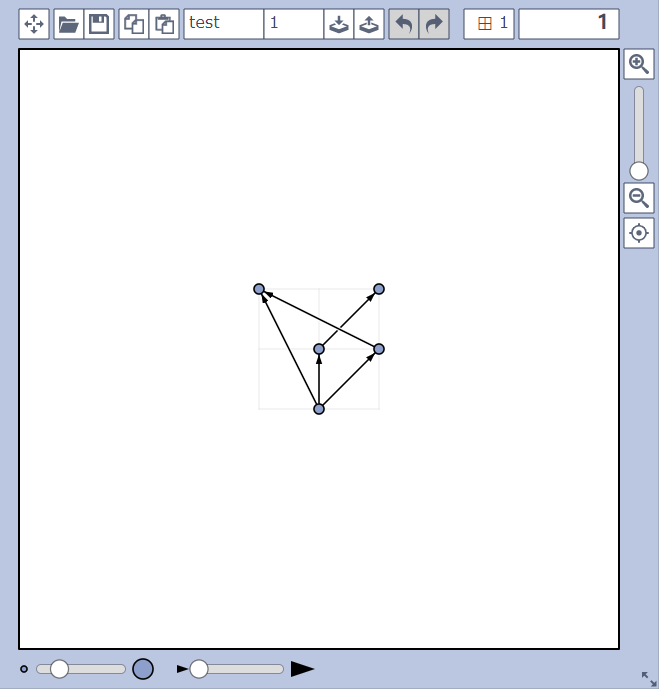
\includegraphics[width=6cm]{graph-1.png}
		%\caption{fig1}
	}
	\quad
	\subfigure[localSearch graph-1]{
		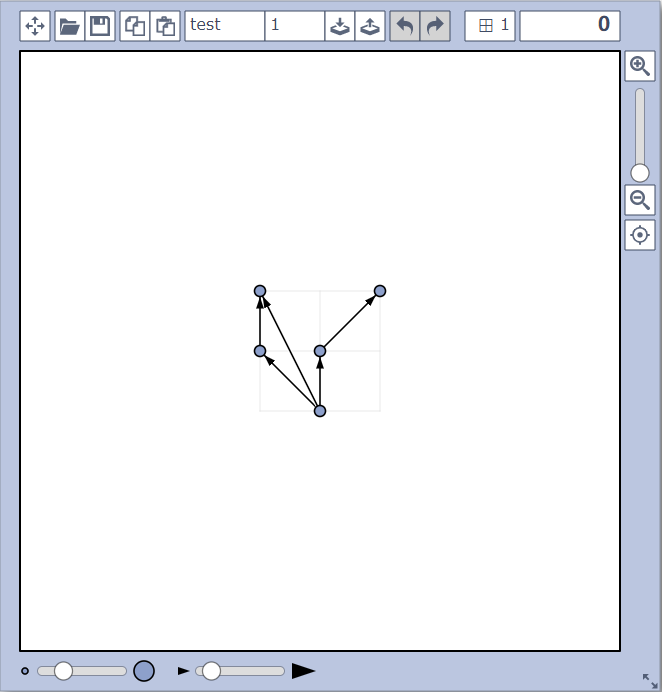
\includegraphics[width=6cm]{test3-graph-1.png}
	}
	\quad
	\subfigure[graph-2]{
		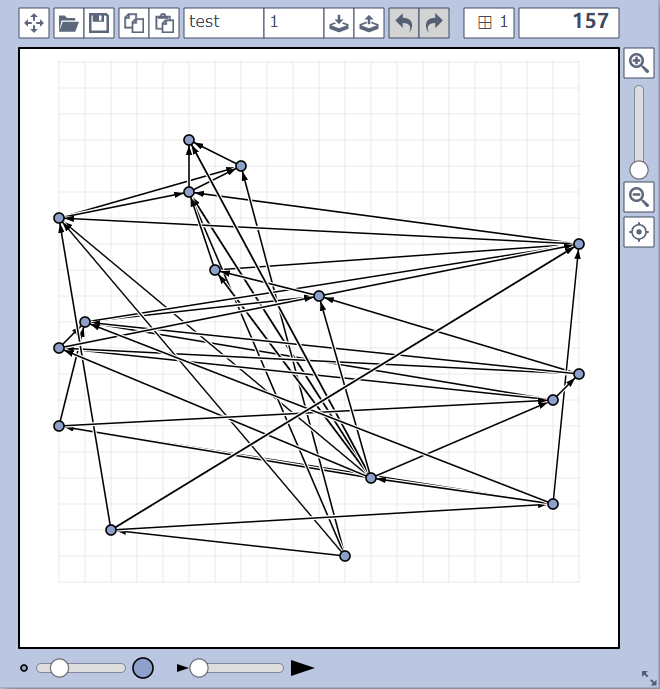
\includegraphics[width=6cm]{graph-2.png}
	}
	\quad
	\subfigure[localSearch graph-2]{
		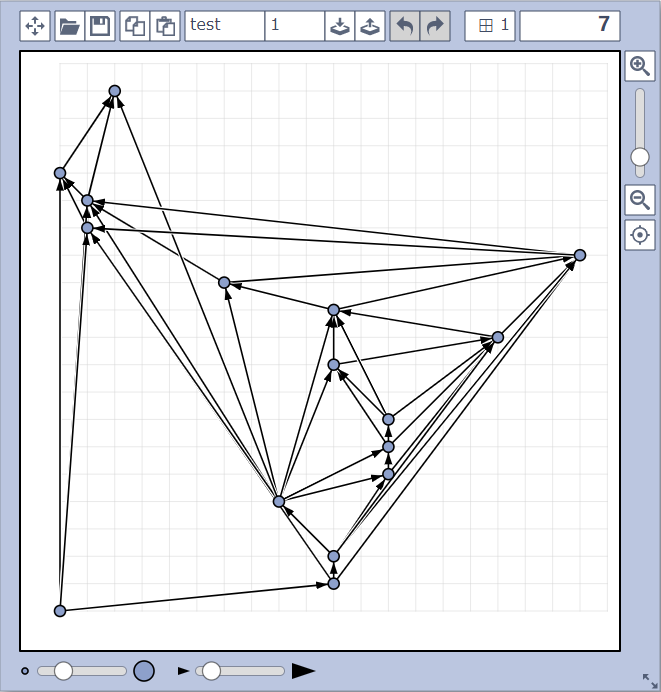
\includegraphics[width=6cm]{test3-graph-2.png}
	}
	\quad
	\subfigure[graph-3]{
		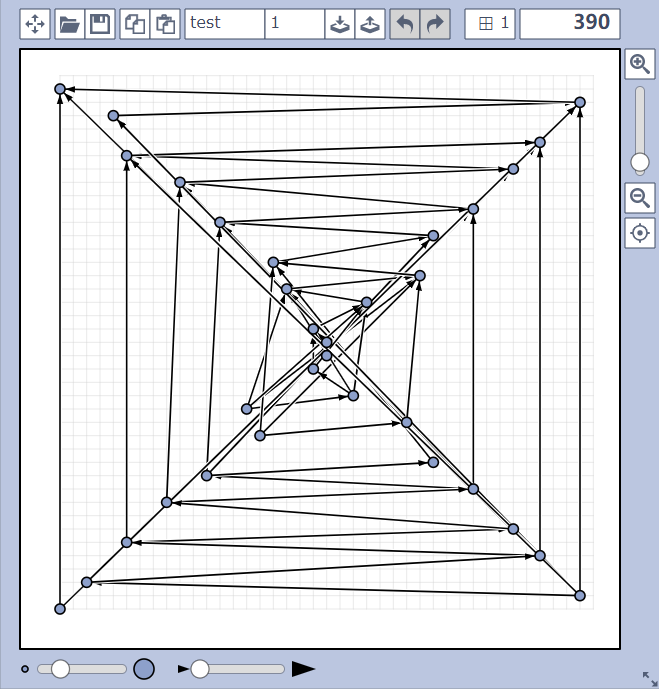
\includegraphics[width=6cm]{graph-3.png}
	}
	\quad
	\subfigure[localSearch graph-3]{
		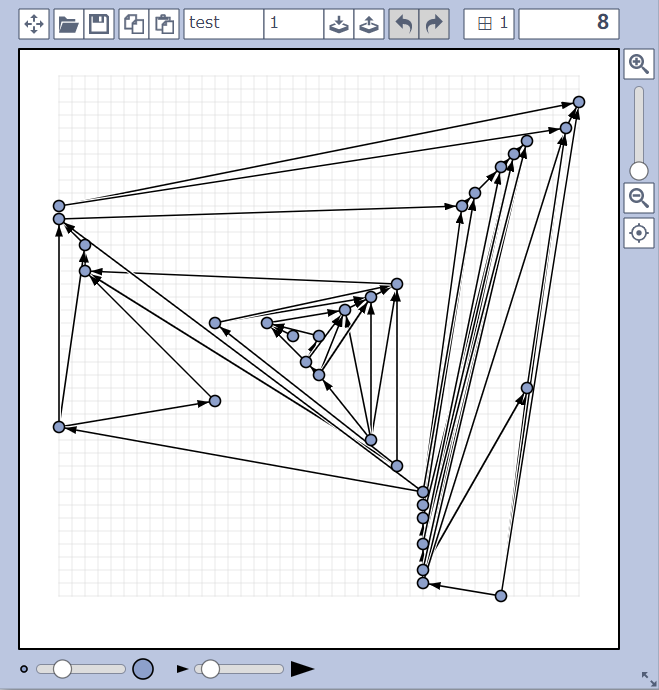
\includegraphics[width=6cm]{test3-graph-3.png}
	}
	\caption{Comparison of initial layout and localSearch output in small input}
	\label{local1}
\end{figure}

\begin{figure}[htbp]
	\centering
	\subfigure[graph-4]{
		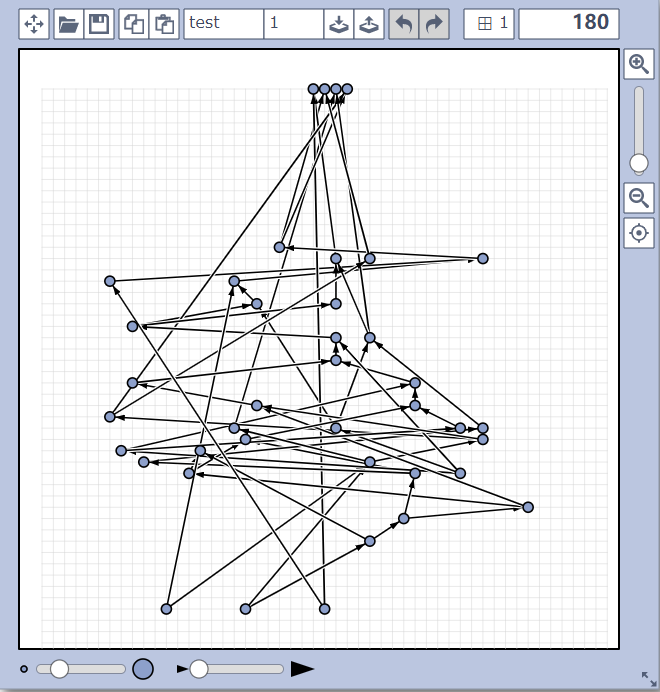
\includegraphics[width=6cm]{graph-4.png}
		%\caption{fig1}
	}
	\quad
	\subfigure[localSearch graph-4]{
		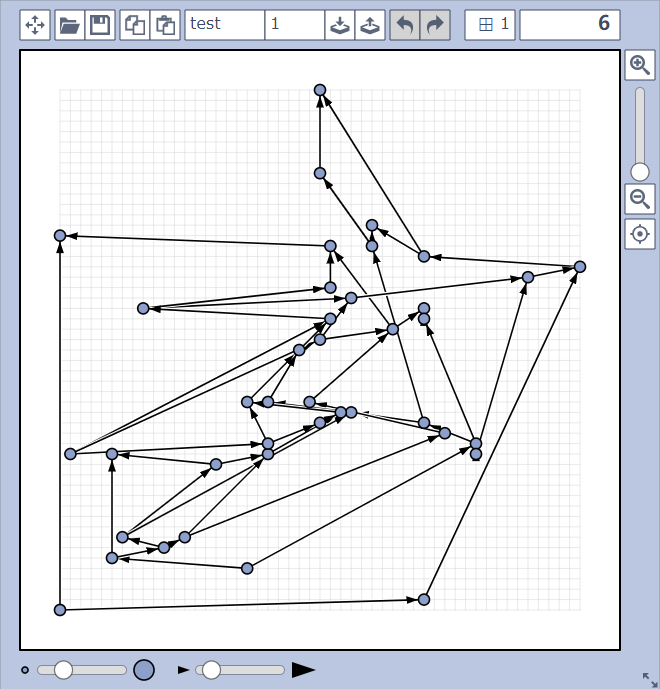
\includegraphics[width=6cm]{test3-graph-4.png}
	}
	\quad
	\subfigure[graph-5]{
		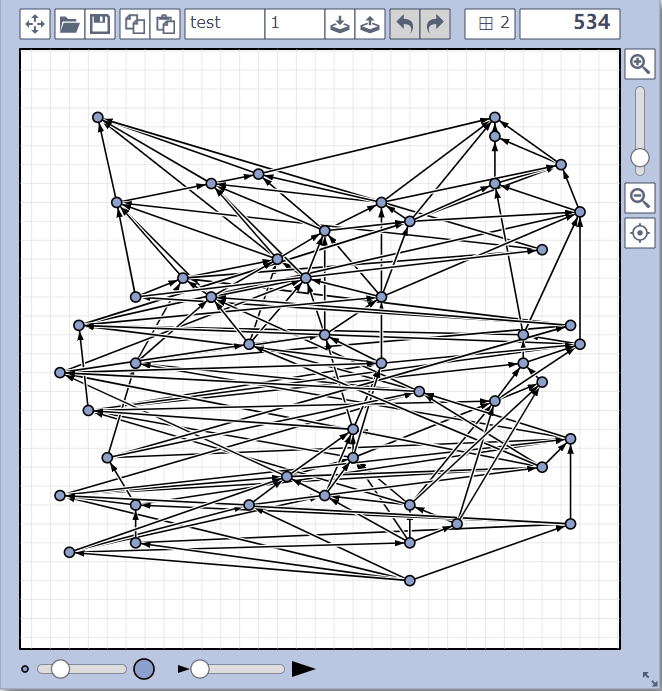
\includegraphics[width=6cm]{graph-5.png}
	}
	\quad
	\subfigure[localSearch graph-5]{
		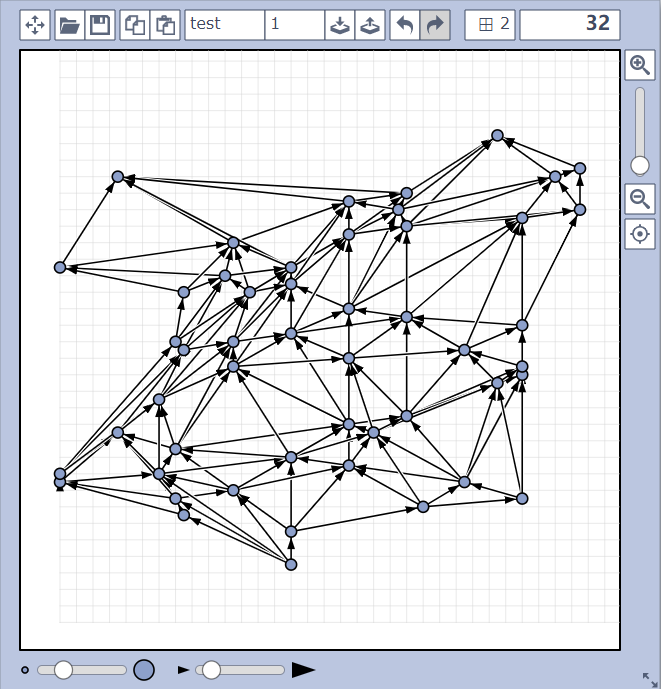
\includegraphics[width=6cm]{test3-graph-5.png}
	}
	\quad
	\subfigure[graph-6]{
		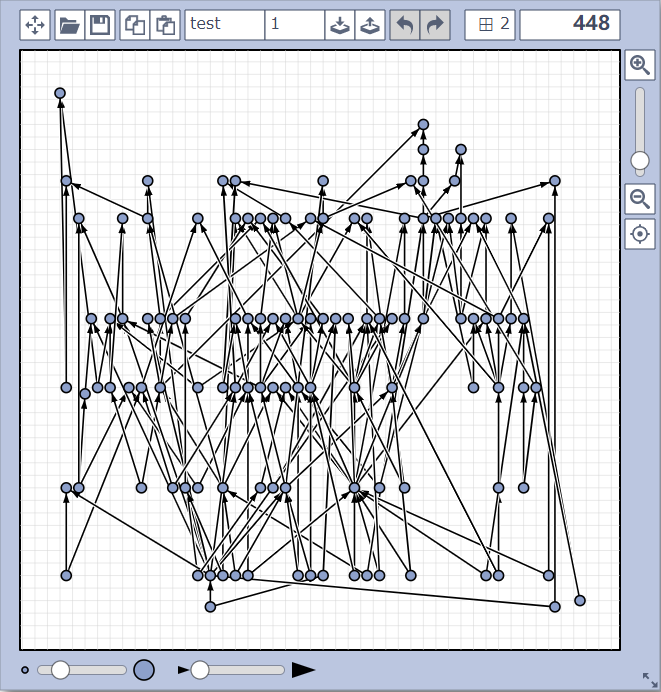
\includegraphics[width=6cm]{graph-6.png}
	}
	\quad
	\subfigure[localSearch graph-6]{
		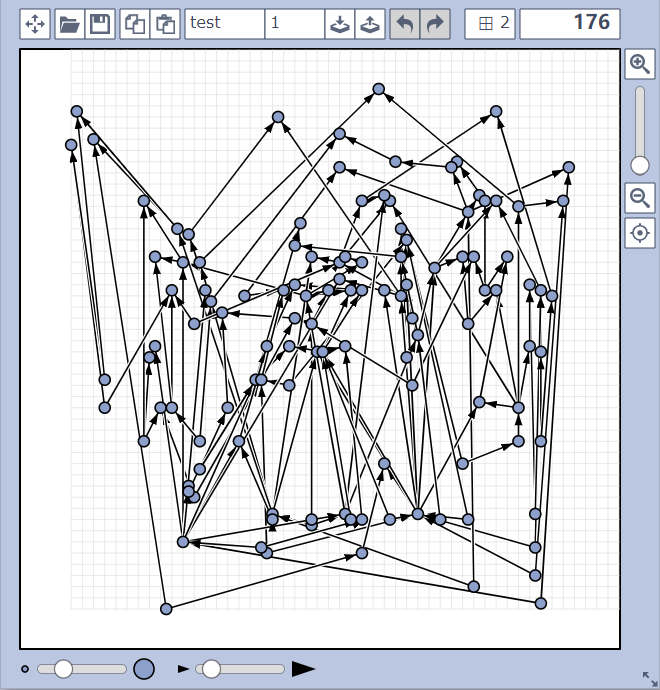
\includegraphics[width=6cm]{test3-graph-6.png}
	}
	\caption{Comparison of initial layout and localSearch output in small input}
	\label{local2}
\end{figure}

\begin{figure}[htbp]
	\centering
	\subfigure[auto-7]{
		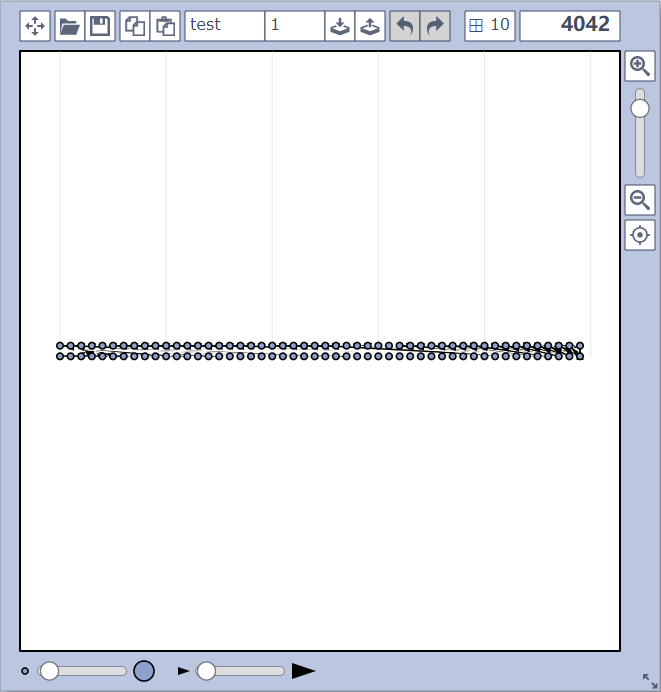
\includegraphics[width=6cm]{auto-7.png}
		%\caption{fig1}
	}
	\quad
	\subfigure[localSearch auto-7]{
		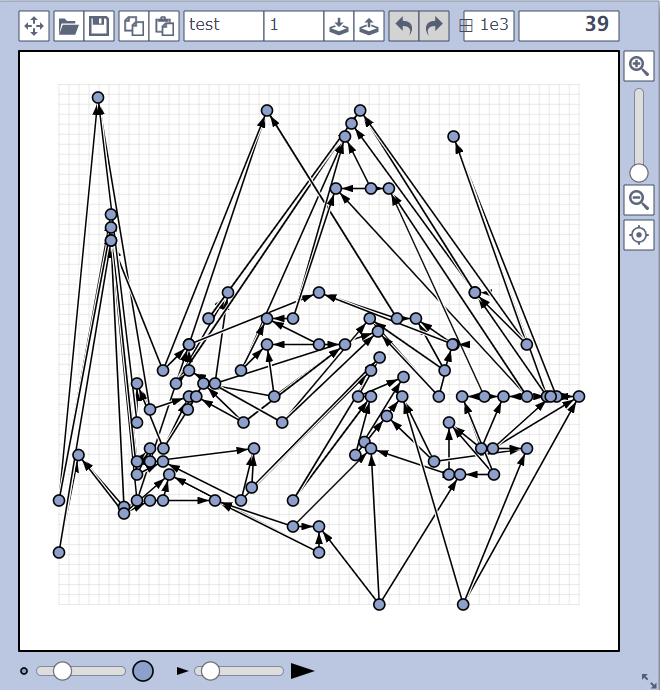
\includegraphics[width=6cm]{test3-auto-7.png}
	}
	\quad
	\subfigure[auto-8]{
		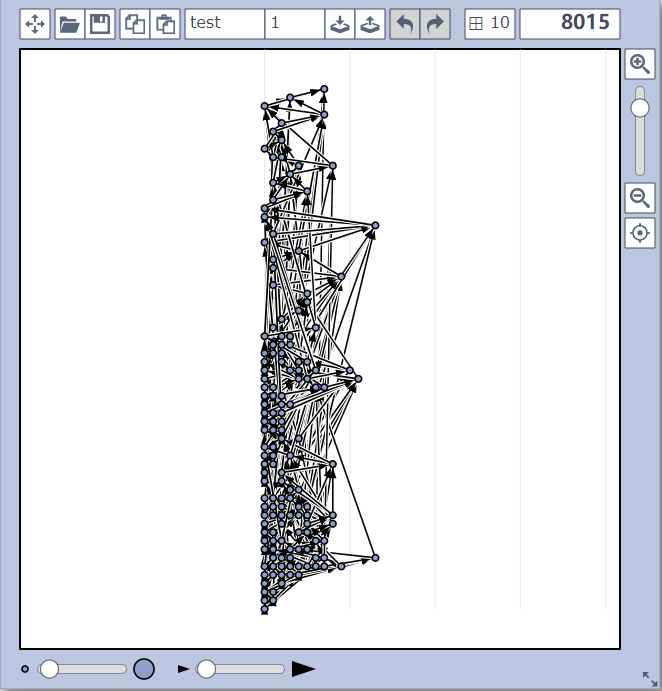
\includegraphics[width=6cm]{auto-8.png}
	}
	\quad
	\subfigure[localSearch auto-8]{
		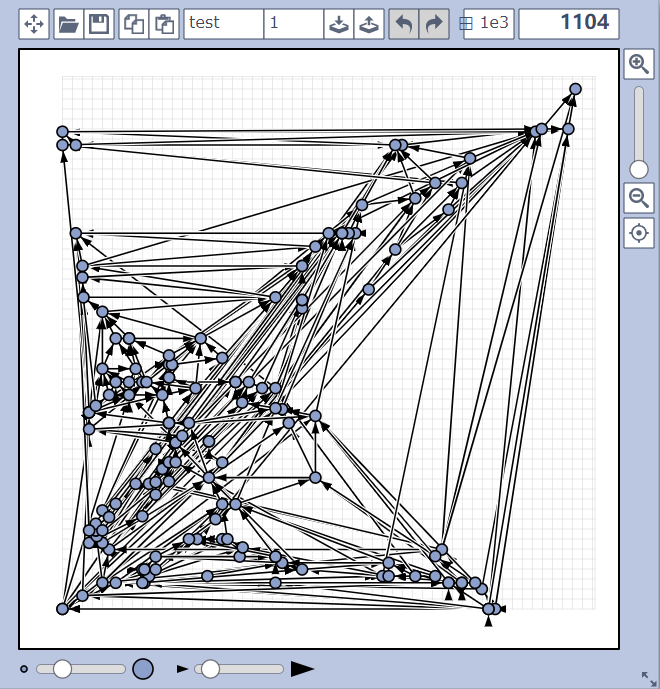
\includegraphics[width=6cm]{test3-auto-8.png}
	}
	\quad
	\subfigure[auto-9]{
		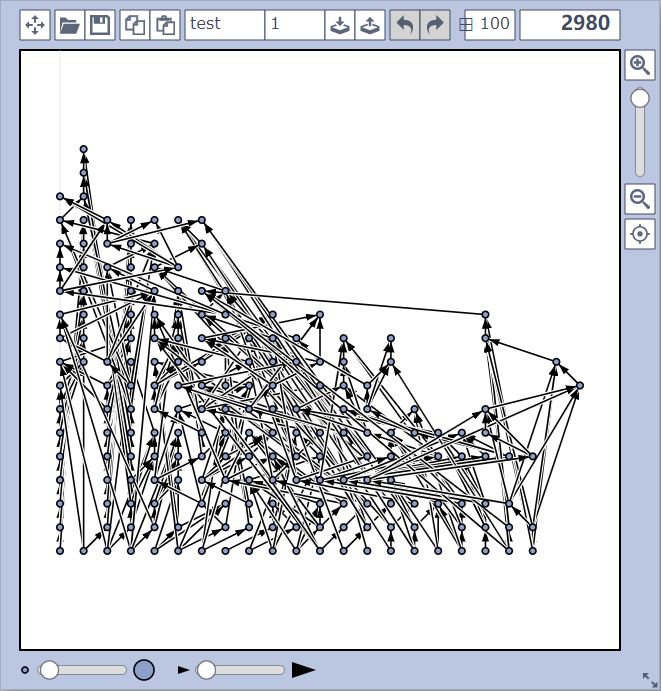
\includegraphics[width=6cm]{auto-9.png}
	}
	\quad
	\subfigure[localSearch auto-9]{
		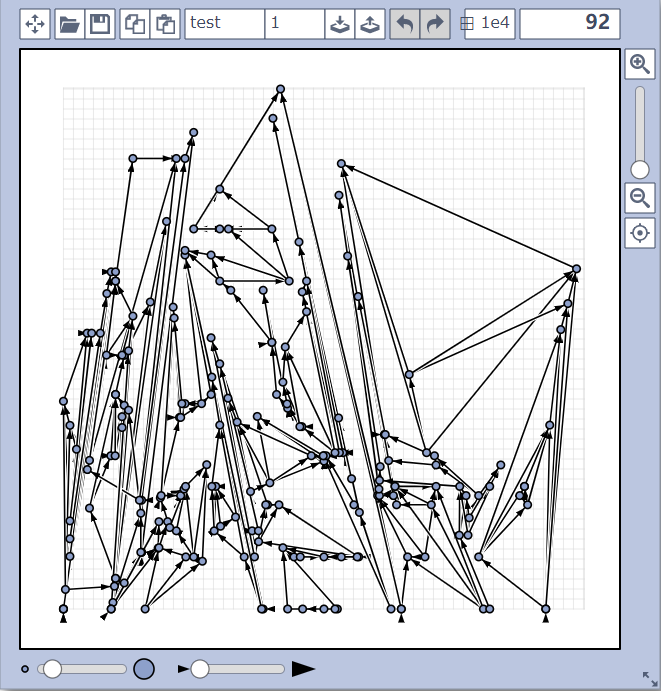
\includegraphics[width=6cm]{test3-auto-9.png}
	}
	\caption{Comparison of initial layout and localSearch output in large input}
	\label{local3}
\end{figure}

\begin{figure}[htbp]
	\centering
	\subfigure[auto-10]{
		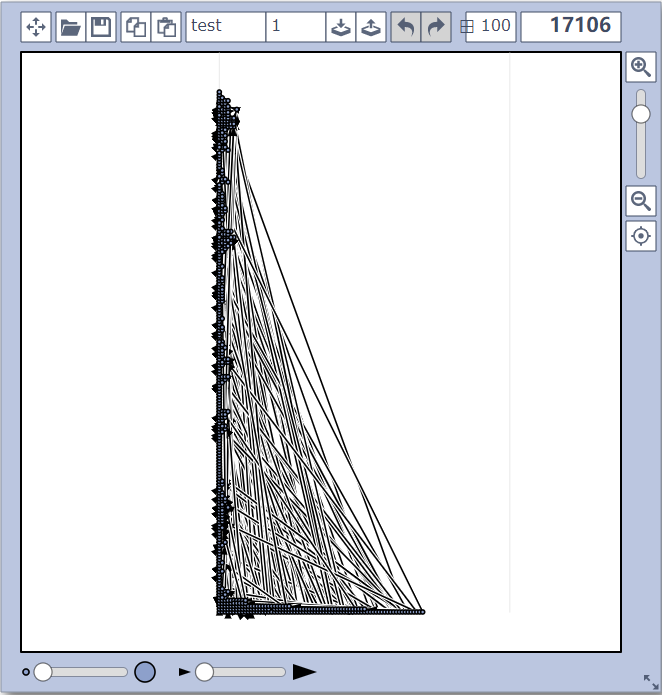
\includegraphics[width=6cm]{auto-10.png}
		%\caption{fig1}
	}
	\quad
	\subfigure[forceDirected auto-10]{
		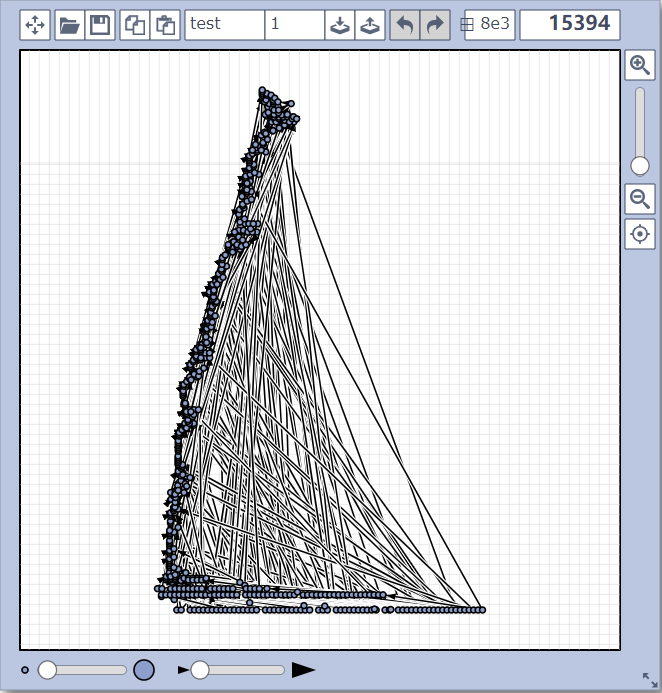
\includegraphics[width=6cm]{test2-auto-10.png}
	}
	\quad
	\subfigure[auto-11]{
		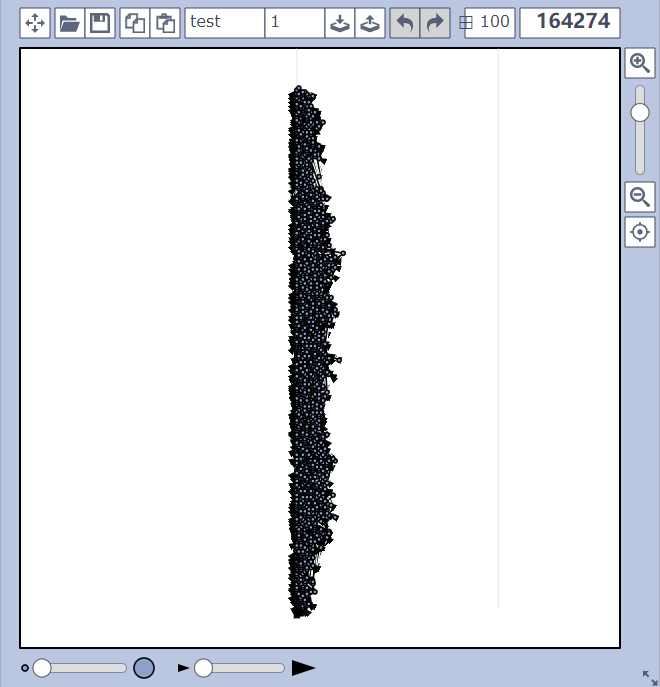
\includegraphics[width=6cm]{auto-11.png}
	}
	\quad
	\subfigure[forceDirected auto-11]{
		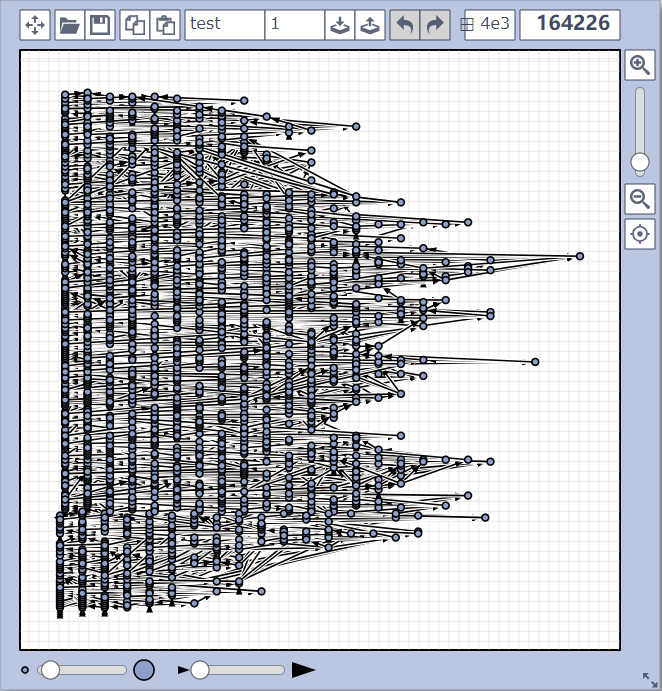
\includegraphics[width=6cm]{test2-auto-11.png}
	}
	\quad
	\subfigure[auto-12]{
		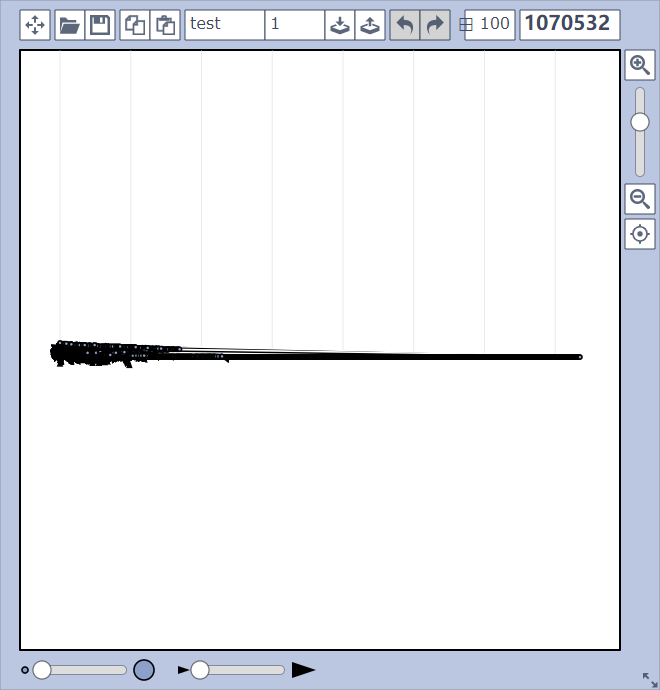
\includegraphics[width=6cm]{auto-12.png}
	}
	\quad
	\subfigure[forceDirected auto-12]{
		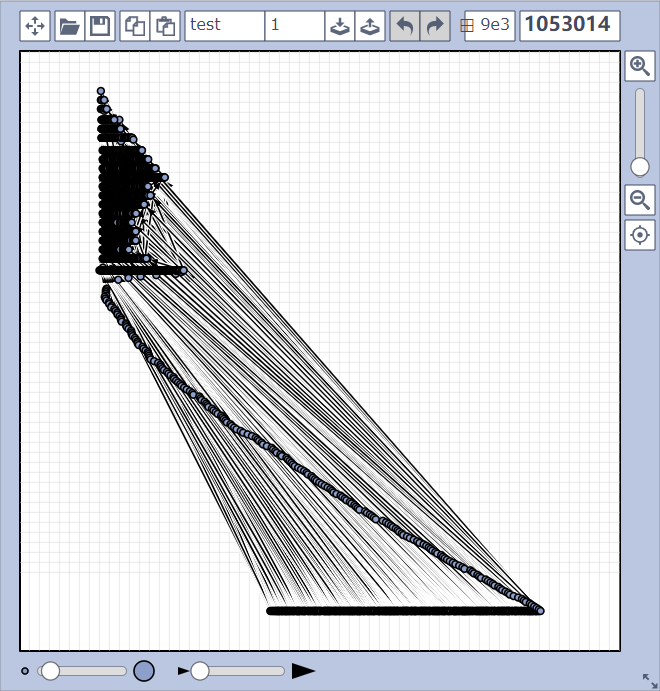
\includegraphics[width=6cm]{test2-auto-12.png}
	}
	\caption{Comparison of initial layout and forceDirected output in large input}
	\label{force1}
\end{figure}

\begin{figure}[htbp]
	\centering
	\subfigure[Initial auto-7]{
		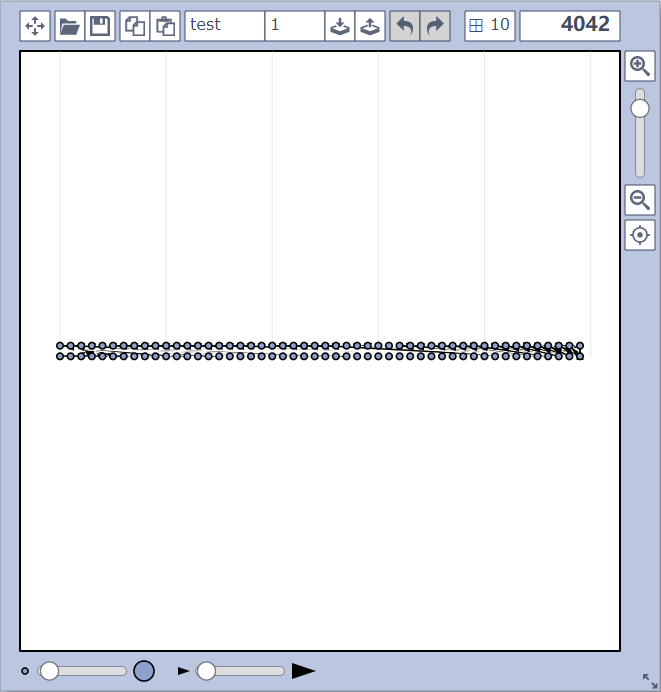
\includegraphics[width=4.7cm]{auto-7.png}
	}
	\quad
	\subfigure[forceDirected auto-7]{
		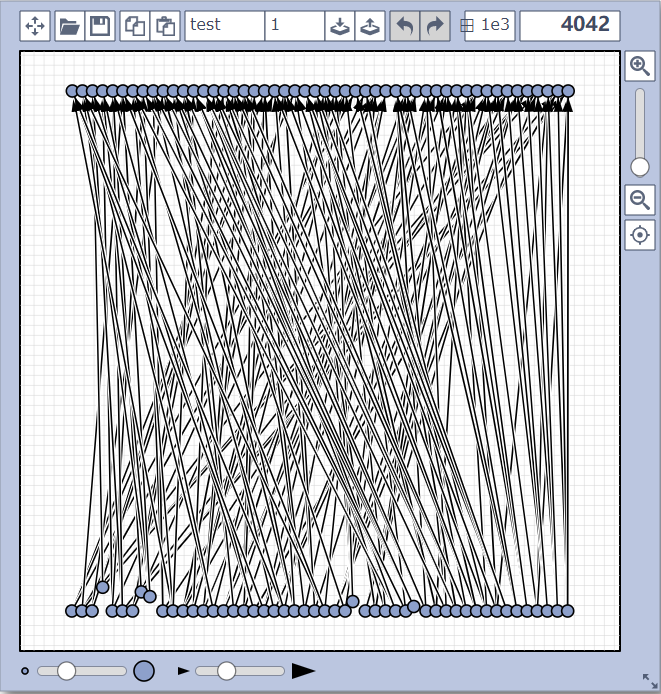
\includegraphics[width=4.7cm]{test2-auto-7.png}
		%\caption{fig1}
	}
	\quad
	\subfigure[localSearch auto-7]{
		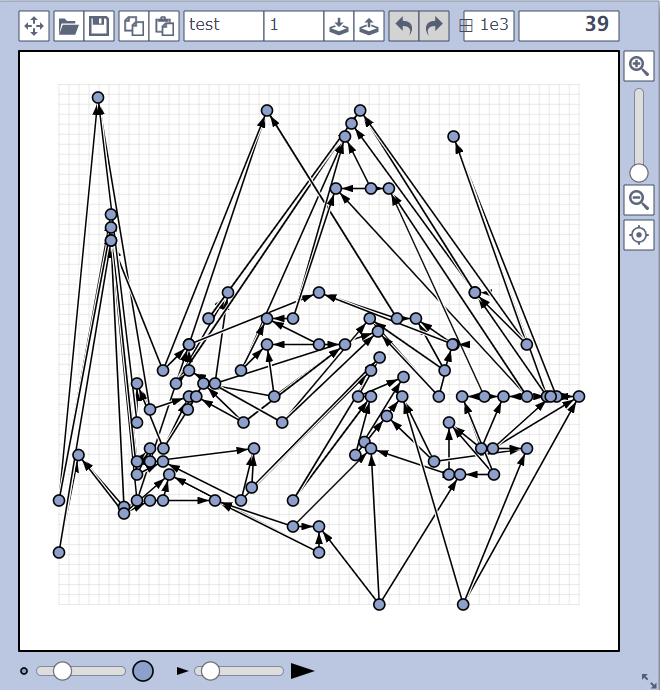
\includegraphics[width=4.7cm]{test3-auto-7.png}
	}
	
	
	\centering
	\subfigure[Initial auto-8]{
		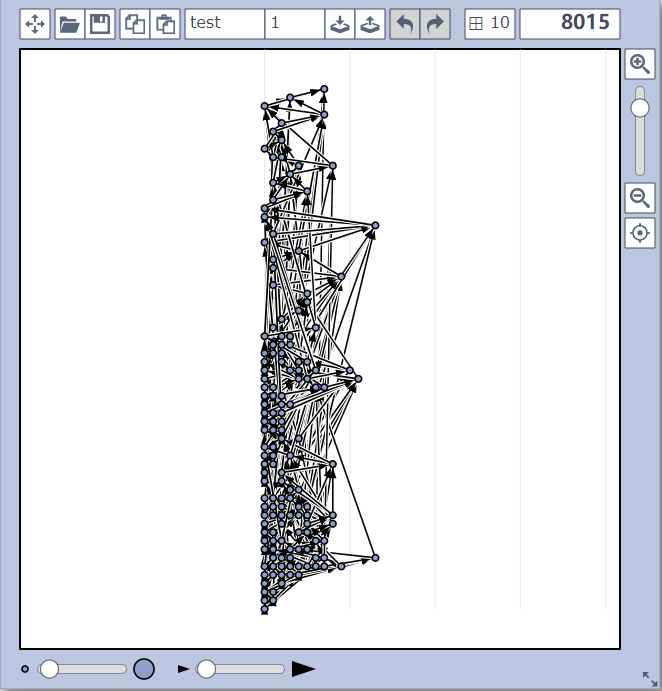
\includegraphics[width=4.7cm]{auto-8.png}
	}
	\quad
	\subfigure[forceDirected auto-8]{
		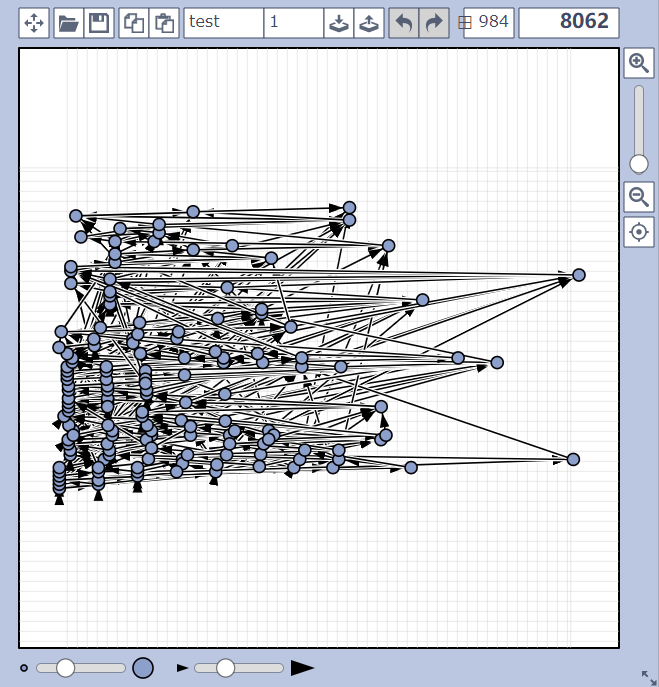
\includegraphics[width=4.7cm]{test2-auto-8.png}
		%\caption{fig1}
	}
	\quad
	\subfigure[localSearch auto-8]{
		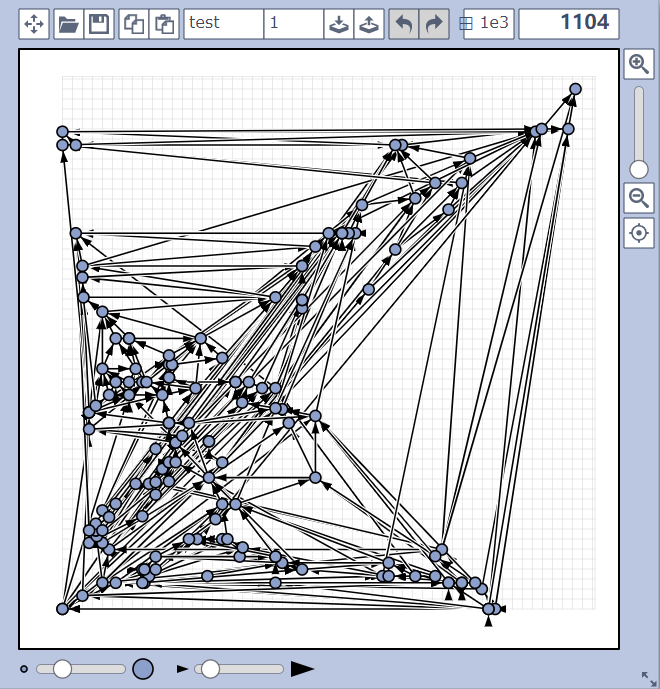
\includegraphics[width=4.7cm]{test3-auto-8.png}
	}
	
	
	\centering
	\subfigure[Initial auto-9]{
		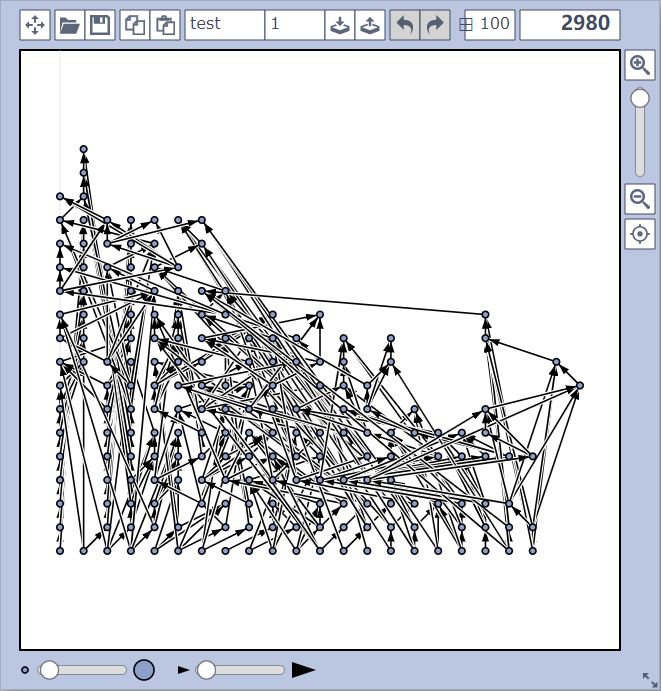
\includegraphics[width=4.7cm]{auto-9.png}
	}
	\quad
	\subfigure[forceDirected auto-9]{
		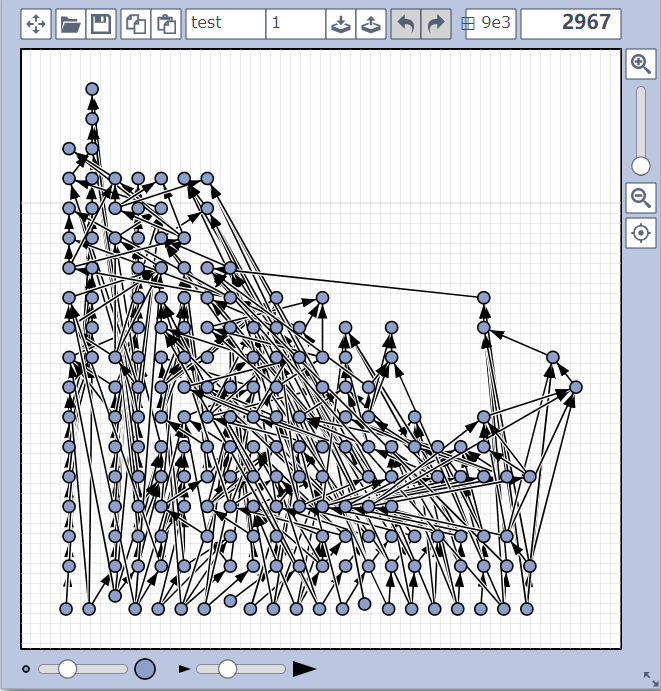
\includegraphics[width=4.7cm]{test2-auto-9.png}
		%\caption{fig1}
	}
	\quad
	\subfigure[localSearch auto-9]{
		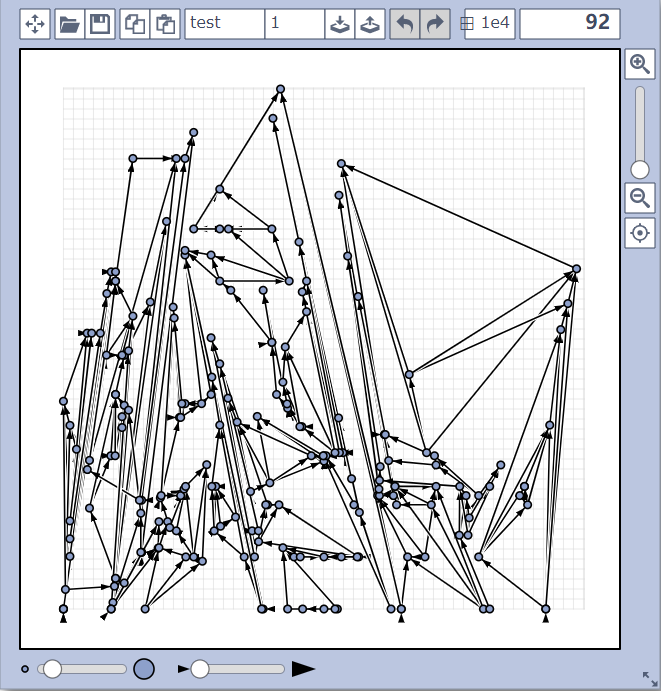
\includegraphics[width=4.7cm]{test3-auto-9.png}
	}
	
	
	\centering
	\subfigure[Initial auto-10]{
		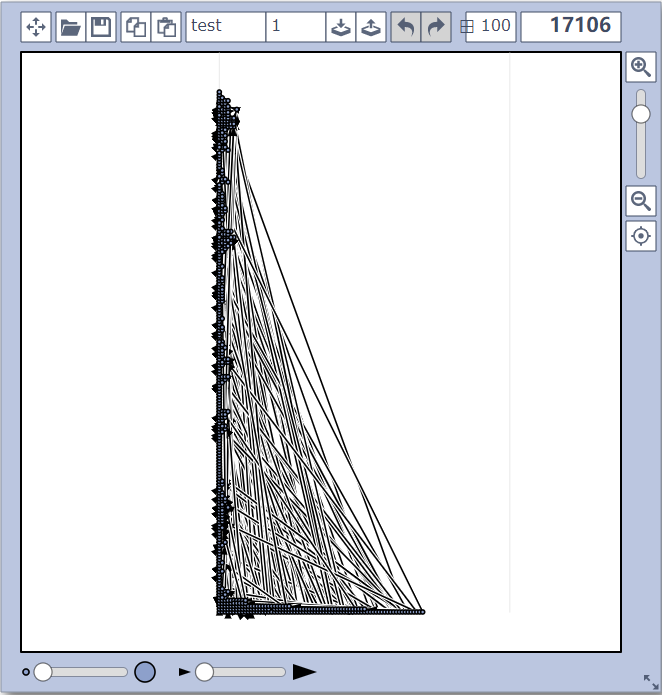
\includegraphics[width=4.7cm]{auto-10.png}
	}
	\quad
	\subfigure[forceDirected auto-10]{
		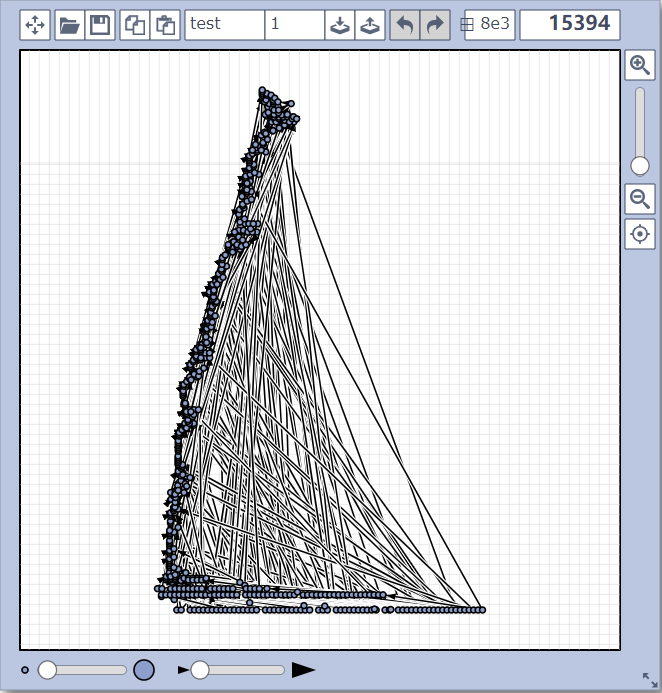
\includegraphics[width=4.7cm]{test2-auto-10.png}
		%\caption{fig1}
	}
	\quad
	\subfigure[localSearch auto-10]{
		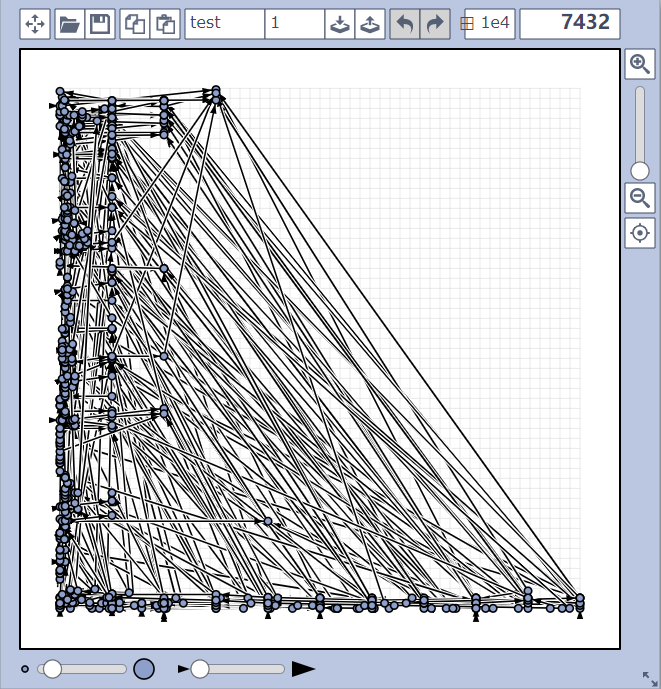
\includegraphics[width=4.7cm]{test3-auto-10.png}
	}
	\caption{Comparison of initial layout, forceDirected output and localSearch output in large input}
	\label{all1}
\end{figure}
\newpage
\subsection{Result Analysis}
For large input, by adding the edge-repulsive force in the force-directed heuristic algorithm, our algorithm works very well
presenting a fast output of valid drawing automatically without a check of validation. However the crossing reduction depends largely on the structure of the graph itself, for some graphs close to complete graphs the result may not be so satisfying.

On the contrary, this algorithm works not so satisfactorily in small input. especially those whose space of valid drawing is close to the space of the whole canvas.

The local search heuristic algorithm presents a highly robust quality both in small input and large input. By setting properly the parameters $C_{step}$ and $C_{range}$, we can obtain a result quite satisfying. However, if the two parameters are not properly chosen, the output may ends at first iteration and returns the original initial output, or it may take a long time to converge towards our final output. Especially in large input, the running time increases rapidly with the input size.


\begin{table}[t]
	\centering  
	\fontsize{6.5}{8}\selectfont  
	\begin{threeparttable}  
		\caption{Performance comparison.}  
		\label{tab:performance_comparison}  
		\begin{tabular}{ccccccc}  
			\toprule  
			\multirow{2}{*}{Original crossing number}&
			\multicolumn{3}{c}{ Force-directed layouts}&\multicolumn{3}{c}{ Local search heuristic}\cr  
			\cmidrule(lr){2-4} \cmidrule(lr){5-7}  
			&Crossing number&Reduction ratio&Runtime(seconds)&Crossing Number&Reduction ratio&Runtime(seconds)\cr  
			\midrule  
			1&$\backslash$&$\backslash$&$\backslash$&0&$100\%$&0.01\cr  
			157&$\backslash$&$\backslash$&$\backslash$&7&$95.5\%$&0.49\cr  
			390&$\backslash$&$\backslash$&$\backslash$&8&$97.9\%$&4.47\cr  
			180&$\backslash$&$\backslash$&$\backslash$&6&$96.7\%$&2.80\cr  
			534&$\backslash$&$\backslash$&$\backslash$&32&$94.0\%$&4.83\cr 448&$\backslash$&$\backslash$&$\backslash$&176&$60.7\%$&4.30\cr 4042&4042&$0.00\%$&0.0767551&39&$99.0\%$&77.6\cr
			8015&8062&$-0.58\%$&0.1362603&1104&$80.1\%$&205\cr
			2980&2967&$0.44\%$&0.3202732&92&$96.9\%$&646\cr
			17106&15394&$10.0\%$&1.0021531&7432&$56.6\%$&900\cr
			164274&164226&$0.03\%$&6.3856798&42083&$25.6\%$&$>10^7$\cr
			1070532&1053014&$1.63\%$&12.2658151&$\backslash$&$\backslash$&$\backslash$\cr
			
			\bottomrule  
		\end{tabular}  
	\end{threeparttable}  
\end{table}  



\end{document}
